%=====================================================================
%  penetrating_divisors.tex
%  Penetrating Divisors: a full computation ledger on P^1_C.
%  Self-contained. Compile with:  latexmk -pdf penetrating_divisors.tex
%  No shell escape, no external images, no nonstandard fonts.
%=====================================================================
\documentclass[11pt]{article}

\usepackage[T1]{fontenc}
\usepackage{lmodern}
\usepackage[a4paper,margin=2.1cm]{geometry}
\usepackage{amsmath,amssymb,amsthm,mathtools}
\usepackage{graphicx}
\usepackage{tikz}
\usepackage{tikz-cd}
\usepackage{xcolor}
\usepackage{enumitem}
\usepackage{array}
\usepackage{booktabs}

\usetikzlibrary{positioning,arrows.meta,calc,decorations.pathmorphing,backgrounds}

%---------------------------------------------------------------------
%  Colors
%---------------------------------------------------------------------
\definecolor{inkblue}{RGB}{22,32,72}
\definecolor{polered}{RGB}{172,28,40}
\definecolor{zerogreen}{RGB}{18,108,72}
\definecolor{accent}{RGB}{176,104,12}
\definecolor{paper}{RGB}{250,248,240}
\definecolor{faint}{RGB}{120,120,132}

%---------------------------------------------------------------------
%  Macros
%---------------------------------------------------------------------
\newcommand{\PP}{\mathbb P}
\newcommand{\CC}{\mathbb C}
\newcommand{\OO}{\mathcal O}
\newcommand{\MM}{\mathcal M}
\newcommand{\Div}{\operatorname{Div}}
\newcommand{\divisor}{\operatorname{div}}
\newcommand{\ord}{\operatorname{ord}}
\newcommand{\Pic}{\operatorname{Pic}}
\newcommand{\Span}{\operatorname{span}}
\newcommand{\AAA}{\mathbb A}

\newcommand{\step}[1]{\smallskip\noindent\textit{\textcolor{accent}{#1}}\ }
\newcommand{\target}[2]{\medskip\noindent%
  {\small\textsc{\textcolor{accent}{Target #1.}}}\ \textbf{\textcolor{inkblue}{#2}}\par\nopagebreak\smallskip}
\newcommand{\warningnote}{\par\smallskip\noindent%
  {\color{polered}\textbf{Warning.}}\ \emph{The raw meromorphic value of a section
  is not the same thing as the value of that section in a local trivialization.}\ }

%---------------------------------------------------------------------
%  Boxed prose
%---------------------------------------------------------------------
\newcommand{\philobox}[1]{%
  \begin{center}\setlength{\fboxrule}{0.8pt}%
  \fcolorbox{inkblue}{paper}{\parbox{0.93\linewidth}{\itshape #1}}\end{center}}
\newcommand{\diagbox}[3]{%
  \begin{center}\setlength{\fboxrule}{1pt}%
  \fcolorbox{accent}{paper}{\parbox{0.9\linewidth}{\small
     \textbf{Probe tests:}\ #1\\[2pt]
     \textbf{It reveals:}\ #2\\[2pt]
     \textbf{Verdict:}\ #3}}\end{center}}

%---------------------------------------------------------------------
%  Divisor strip on P^1 (geometry of the support)
%---------------------------------------------------------------------
\newcommand{\probeline}[3]{%
\begin{center}
\begin{tikzpicture}[x=1.5cm,y=1cm,baseline]
  \draw[inkblue, line width=0.9pt, -{Stealth[length=2.2mm]}] (-0.6,0) -- (4.3,0);
  \node[inkblue] at (4.7,0) {$\PP^1$};
  \foreach \px in {0,2,4}{\fill[inkblue] (\px,0) circle (1.6pt);}
  \node[inkblue, below=3pt] at (0,0) {$0$};
  \node[inkblue, below=3pt] at (2,0) {$1$};
  \node[inkblue, below=3pt] at (4,0) {$\infty$};
  #1 #2
\end{tikzpicture}\\[3pt]
{\footnotesize\textcolor{faint}{#3}}
\end{center}}

%---------------------------------------------------------------------
%  Per-probe COMMUTATIVE LADDER
%   top rail (global): D -> L(D) = H^0 -> basis -> Phi_D
%   bottom rail (local): D -> Cartier -> g_ab -> line bundle
%   keystone sheaf O(D); blue arrows = constructions, amber rungs = identifications.
% #1 D  #2 O(D)  #3 line bundle  #4 g  #5 Cartier  #6 L(D)  #7 H^0  #8 basis  #9 map
%---------------------------------------------------------------------
\tikzset{
  mapnode/.style={draw=inkblue, line width=0.7pt, rounded corners=2pt, fill=paper,
                  inner sep=4pt, align=center, font=\small, text=inkblue},
  centernode/.style={draw=polered, line width=1.3pt, rounded corners=3pt, fill=paper,
                  inner sep=6pt, align=center, font=\bfseries, text=inkblue},
  maparrow/.style={-{Stealth[length=2.6mm]}, inkblue, line width=0.8pt},
  rimarrow/.style={-{Stealth[length=2.6mm]}, accent, line width=0.85pt},
  identrung/.style={accent, line width=0.7pt, double, double distance=1.3pt},
  arrlbl/.style={font=\scriptsize\itshape, text=faint, align=center, fill=paper, inner sep=1.5pt},
  rimlbl/.style={font=\scriptsize\itshape, text=accent, align=center, fill=paper, inner sep=1.5pt}
}
\newcommand{\probemap}[9]{%
\begin{center}
\resizebox{0.97\textwidth}{!}{%
\begin{tikzpicture}
  \node[centernode] (D)   at (0,0)     {#1};
  \node[mapnode] (LD)  at (3.5,1.75)   {#6};
  \node[mapnode] (H0)  at (7.1,1.75)   {#7};
  \node[mapnode] (BAS) at (10.6,1.75)  {#8};
  \node[mapnode] (CAR) at (3.5,-1.75)  {#5};
  \node[mapnode] (GIJ) at (7.1,-1.75)  {#4};
  \node[mapnode] (BUN) at (10.6,-1.75) {#3};
  \node[mapnode] (OD)  at (8.5,0)       {#2};
  \node[mapnode] (PHI) at (13.5,0)      {#9};
  \draw[maparrow] (D)   -- node[arrlbl,pos=0.55]{allow \&\\ force} (LD);
  \draw[maparrow] (D)   -- node[arrlbl,pos=0.55]{local\\ eqns $f_\alpha$} (CAR);
  \draw[maparrow] (H0)  -- node[arrlbl]{pick a\\ basis} (BAS);
  \draw[maparrow] (CAR) -- node[arrlbl]{$f_\beta/f_\alpha$} (GIJ);
  \draw[maparrow] (GIJ) -- node[arrlbl]{glue\\ $U_\alpha\!\times\!\CC$} (BUN);
  \draw[maparrow] (BAS) -- node[arrlbl,pos=0.6]{$[s_0\!:\!\cdots\!:\!s_r]$} (PHI);
  \draw[maparrow] (BUN) -- node[arrlbl,pos=0.6]{$|D|$} (PHI);
  \draw[identrung] (LD) -- node[rimlbl]{$=$} (H0);
  \draw[identrung] (H0) -- node[rimlbl,pos=0.55]{$\Gamma$: global\\ sections} (OD);
  \draw[identrung] (OD) -- node[rimlbl,pos=0.5]{$\cong$ sheaf of\\ sections} (BUN);
\end{tikzpicture}}
\end{center}}

%---------------------------------------------------------------------
\theoremstyle{plain}
\newtheorem{proposition}{Proposition}
\theoremstyle{definition}
\newtheorem{remark}{Remark}

\setlist[enumerate]{leftmargin=2.0em, itemsep=2pt, topsep=3pt}
\setlist[itemize]{leftmargin=1.6em, itemsep=2pt, topsep=3pt}

%---------------------------------------------------------------------
\title{\bfseries Penetrating Divisors: A Full Computation Ledger\\[3pt]
       \large Zeros and Poles as Diagnostic Instruments on \(\PP^1_\CC\)}
\author{\textsc{A Computation-First Atlas}}
\date{\today}
%---------------------------------------------------------------------

\begin{document}
\maketitle

\begin{center}\itshape\small
Every abstract object tied back to concrete local equations, valuations, bases,
transition functions, and section evaluations: divisors, $L(D)$, $\OO(D)$,
Cartier data, line bundles, $H^0$, base points, and projective maps, computed in
full.
\end{center}

\medskip
\philobox{A divisor is not merely a formal sum of points. A divisor is a
diagnostic instrument. By placing poles where we wish to permit blow-up and
zeros where we wish to force vanishing, we interrogate a curve and compel its
geometry to answer. This document is a ledger: for each probe we do not assert
what the targets are --- we \emph{compute} them, step by step, from the divisor.}

%=====================================================================
\section{The Situation and Its Targets}
%=====================================================================
\noindent\textbf{The situation.}
We analyze the complex projective line $X=\PP^1_{\CC}$, covered by the two
standard affine charts
\[
  U_0=\PP^1\setminus\{\infty\}\ \text{(coordinate } z\text{)},\qquad
  U_1=\PP^1\setminus\{0\}\ \text{(coordinate } w=\tfrac1z\text{)},
\]
with overlap $U_0\cap U_1=\CC^\times$. The local coordinate at a finite point
$a$ is $t_a=z-a$; at $\infty$ it is $t_\infty=w$. For a rational function
$f=N(z)/M(z)$ in lowest terms,
\[
  \ord_a(f)=\ord_a N-\ord_a M\ \ (a\ \text{finite}),\qquad
  \ord_\infty(f)=\deg M-\deg N .
\]
We probe $X$ with divisors supported in $\{0,\infty\}$, so each support point is
the center of exactly one chart and the two-chart cover is automatically adapted
to the support (see the remark below).

\begin{remark}[Stated assumptions]\label{rmk:assume}
The situation slot was delivered empty. To honour the requirement that every
quantity be \emph{computed}, we fix $X=\PP^1_\CC$ --- the setting where $L(D)$,
$\OO(D)$, Cartier data, transition functions, and projective maps all admit
closed-form rational answers. We further place all supports in $\{0,\infty\}$;
then the support-adapted cover prescribed in general (an open $U_0=X\setminus
\operatorname{Supp}D$ together with disks $U_p$ around each $p$, with local
equation $f_p=t_p^{\,n_p}$) coincides with the two affine charts: the chart
$U_0$ carries the support at $0$ via $f_0=z^{\,n_0}=t_0^{\,n_0}$, and the chart
$U_1$ carries the support at $\infty$ via $f_1=w^{\,n_\infty}=t_\infty^{\,n_\infty}$.
This keeps every transition function a single monomial.
\end{remark}

\medskip\noindent\textbf{The targets.}
For each divisor we expose, in order:
\begin{enumerate}
  \item the divisor $D$ itself, read as valuation inequalities;
  \item the Riemann--Roch space $L(D)$ with an explicit basis;
  \item the invertible sheaf $\OO(D)$;
  \item the Cartier local equations $f_\alpha$;
  \item the transition functions $g_{\alpha\beta}=f_\beta/f_\alpha$;
  \item the associated holomorphic line bundle;
  \item the global sections $H^0(X,\OO(D))$ and their local representatives;
  \item the base points of the linear system $|D|$;
  \item the projective map $\Phi_D$;
  \item separation of points and tangent directions.
\end{enumerate}
Each probe receives a \emph{full calculation ledger} computing all ten targets
explicitly. Nothing is asserted that is not first computed.

%=====================================================================
\section{Selection of Penetrating Divisors}
%=====================================================================
The probes are ordered by degree, sweeping from below the floor of visibility up
to a genuine embedding, and ending with the one experiment a \emph{complete}
linear system on $\PP^1$ can never perform.

\begin{description}[leftmargin=0pt,style=unboxed,itemsep=4pt]
  \item[\textcolor{polered}{Probe A: the void.}]\ $D_1=-[0]$ \;(degree $-1$).
        What does a \emph{negative} divisor do to global sections? It forbids
        everything. Tests whether $H^0$ can be empty.
  \item[\textcolor{inkblue}{Probe B: the collapse.}]\ $D_2=[\infty]-[0]$
        \;(degree $0$, nonzero). Exposes linear equivalence $\OO(D_2)\cong\OO$
        and the gap between a \emph{raw value} and a \emph{trivialized section
        value}.
  \item[\textcolor{zerogreen}{Probe C: the minimal embedding.}]\ $D_3=[\infty]$
        \;(degree $1$). Realizes $\OO(1)$ as very ample and embeds $\PP^1$ as a
        line.
  \item[\textcolor{zerogreen}{Probe D: the conic.}]\ $D_4=2[\infty]$
        \;(degree $2$). Embeds $\PP^1$ as a smooth conic in $\PP^2$ (the
        rational normal curve); tests separation of points \emph{and} tangents.
  \item[\textcolor{accent}{Probe E: the incomplete cut.}]\ subsystems
        $V\subsetneq H^0(\PP^1,\OO(2[\infty]))$. Manufactures the two failures a
        complete system on $\PP^1$ cannot show: a \emph{base point} and a
        \emph{failure to separate points}.
\end{description}

%=====================================================================
\section{The Calculation Protocol and Common Machinery}
%=====================================================================
Each ledger executes Targets~1--10 of Section~1. Two computations recur in every
probe, so we record them once.

\step{Uniform Cartier data and transition function.}
For $D=a[0]+b[\infty]$ with $d:=\deg D=a+b$, the support-adapted equations are
\[
  f_0=z^{\,a}\ \text{on }U_0,\qquad f_1=w^{\,b}\ \text{on }U_1 .
\]
On the overlap $\CC^\times$, using $w=1/z$,
\[
  \frac{f_0}{f_1}=\frac{z^{a}}{w^{b}}=z^{a}\,z^{b}=z^{\,a+b}=z^{\,d},
  \qquad
  g_{01}=\frac{f_1}{f_0}=z^{-d}=w^{\,d}\in\OO^\times(\CC^\times),
\]
because the only zero/pole of $z^{d}$ sits at $z=0$ or $z=\infty$, both deleted
from $\CC^\times$. Hence $\OO(D)\cong\OO(d)$.

\step{Riemann--Roch on $\PP^1$.}
Here $g=0$ and the canonical divisor is $K=-2[\infty]$ ($\deg K=2g-2=-2$), so
\[
  \ell(D)-\ell(K-D)=\deg D+1-g=\deg D+1 .
\]
If $\deg D\ge-1$ then $\deg(K-D)=-2-\deg D\le-1<0$, forcing $\ell(K-D)=0$ and
\[
  \boxed{\;\ell(D)=\deg D+1\quad(\deg D\ge-1)\;}, \qquad
  \ell(D)=0\ \ (\deg D<0).
\]
Every ledger cross-checks this count against the basis it derives.

%=====================================================================
\section{Full Calculation Ledgers}
%=====================================================================

%---------------------------------------------------------------------
\subsection*{Full Calculation Ledger for \(D_1=-[0]\)}
%---------------------------------------------------------------------
\probeline{\node[zerogreen,above=3pt,font=\bfseries] at (0,0){$-1$};}{}%
{$D_1=-[0]$: one forced zero at $z=0$; no pole permitted anywhere; $\deg D_1=-1$.}

\target{1}{The divisor itself}
\(D_1=(-1)\,[0]=\sum_p n_p[p]\) with $n_0=-1$ and $n_p=0$ otherwise. The
defining inequality $\divisor(f)+D_1\ge0$ is read pointwise as
$\ord_p(f)+n_p\ge0$:
\begin{center}\small
\begin{tabular}{cccl}
\toprule
point $p$ & coeff.\ $n_p$ & condition $\ord_p(f)+n_p\ge0$ & meaning\\
\midrule
$0$        & $-1$ & $\ord_0(f)\ge 1$       & $f$ must vanish to order $\ge1$ at $0$\\
$\infty$   & $0$  & $\ord_\infty(f)\ge 0$  & $f$ holomorphic at $\infty$\\
other $p$  & $0$  & $\ord_p(f)\ge 0$       & $f$ holomorphic at $p$\\
\bottomrule
\end{tabular}
\end{center}
\(\deg D_1=\sum_p n_p=-1.\)

\target{2}{The Riemann--Roch space \(L(D_1)\)}
By the table, $f\in L(D_1)$ is holomorphic at every point of $\PP^1$ (no poles
anywhere) and vanishes at $0$. A function holomorphic on all of the compact
$\PP^1$ is constant; the only constant with $\ord_0\ge1$ is $0$. Hence
\[
  L(D_1)=\{f\in\CC(z):\ord_0(f)\ge1,\ \ord_p(f)\ge0\ \forall p\}=\{0\},
  \qquad \ell(D_1)=0 .
\]
\emph{Riemann--Roch check.} $K-D_1=-2[\infty]+[0]$ has degree $-1<0$, so
$\ell(K-D_1)=0$ and $\ell(D_1)=\deg D_1+1=0$. Exact. There is no basis to tabulate.

\target{3}{The sheaf \(\OO(D_1)\)}
$\OO(D_1)(U)=\{f\in\MM(U):\divisor(f)+D_1|_U\ge0\}$. Locally:
\begin{itemize}
  \item near $0$ (negative coefficient): sections are forced to vanish,
        $\OO(D_1)(U_0^{\mathrm{sm}})=\{f:\ord_0(f)\ge1\}=z\cdot\OO_{0}$, the
        maximal ideal $\mathfrak m_0$;
  \item away from $0$ (e.g.\ near $\infty$ or any $p\neq0$): no condition,
        $\OO(D_1)(U)=\OO(U)$.
\end{itemize}
Taking $U=X$ reproduces Target~2: $H^0(X,\OO(D_1))=\OO(D_1)(X)=L(D_1)=0$, since a
global section is exactly a global meromorphic function meeting every valuation
inequality of $D_1$.

\target{4}{Cartier data}
Here $a=n_0=-1,\ b=n_\infty=0$, so
\[
  f_0=z^{-1}\ \text{on }U_0,\qquad f_1=w^{0}=1\ \text{on }U_1 .
\]
Check $\divisor(f_0)|_{U_0}$: $z^{-1}$ has a single pole at $z=0$ and no other
zero/pole in $U_0$, so $\divisor(z^{-1})|_{U_0}=-[0]=D_1|_{U_0}$. Check
$\divisor(f_1)|_{U_1}$: $0\notin U_1$, so $D_1|_{U_1}=0=\divisor(1)$. On the
overlap,
\[
  \frac{f_0}{f_1}=z^{-1},
\]
whose pole ($z=0$) and zero ($z=\infty$) both lie outside $\CC^\times$; hence
$f_0/f_1\in\OO^\times(\CC^\times)$.

\target{5}{Transition functions}
Local generators $e_\alpha=f_\alpha^{-1}$:
\[
  e_0=f_0^{-1}=z,\qquad e_1=f_1^{-1}=1 .
\]
From $e_0=(f_1/f_0)e_1$ the transition function is
\[
  g_{01}=\frac{f_1}{f_0}=\frac{1}{z^{-1}}=z=w^{-1}\quad(=z^{-d}\text{ with }d=-1).
\]
With only two charts the cocycle conditions are $g_{00}=g_{11}=1$ and
$g_{10}=f_0/f_1=z^{-1}=g_{01}^{-1}$; triple overlaps are empty, so the cocycle
identity $g_{\alpha\beta}g_{\beta\gamma}=g_{\alpha\gamma}$ holds vacuously.

\target{6}{Invertible sheaf and line bundle}
$\OO(D_1)|_{U_0}=\OO_{U_0}\,e_0$ and $\OO(D_1)|_{U_1}=\OO_{U_1}\,e_1$ are free of
rank $1$. The line bundle $L_1\to\PP^1$ is $U_0\times\CC$ glued to $U_1\times\CC$
by $v_0=g_{01}v_1=z\,v_1$; this is $\OO(-1)$, the tautological bundle.
\emph{Linear equivalence:} with $h=1/z$, $\divisor(h)=\divisor(1/z)=[\infty]-[0]$,
so $D_1-(-[\infty])=-[0]+[\infty]=\divisor(1/z)$, giving $D_1\sim-[\infty]$ and
again $\OO(D_1)\cong\OO(-1)$.

\target{7}{Global sections and local representatives}
$H^0=0$, so there is no nonzero section to trivialize. The mechanism is visible
in the generators: $e_0=z$ is holomorphic on $U_0$, but read on $U_1$ it is
$e_0=z=w^{-1}$, which has a pole at $w=0$ ($z=\infty$). No nonzero constant
multiple of $e_0$ extends across $U_1$, which is exactly why the global section
space is empty.

\target{8}{Base points}
The complete linear system $|D_1|=\{E\ge0:E\sim D_1\}$ is \emph{empty}: any
$E\sim D_1$ has $\deg E=\deg D_1=-1<0$, impossible for an effective divisor.
Equivalently $\dim H^0=0$. There is no section, hence no well-defined base-point
test; conventionally every point is a (trivial) base point of the empty system.

\target{9}{Projective map}
Since $\dim H^0(X,\OO(D_1))=0<2$, no map to any $\PP^{r}$ is defined.

\target{10}{Separation of points and tangent directions}
Not applicable: there is no morphism. The probe's content is precisely the
\emph{absence} of all downstream structure once $\deg D<0$.

\probemap
  {$D_1=-[0]$}
  {$\OO(D_1)\cong\OO(-1)$}
  {line bundle\\ \scriptsize $g_{01}=z$}
  {$g_{01}=z=w^{-1}$}
  {$f_0=z^{-1},\ f_1=1$}
  {$L(D_1)=0$\\ \scriptsize $\ell=0$}
  {$H^0(\OO(D_1))=0$}
  {basis $=\varnothing$}
  {no map\\ \scriptsize ($\ell<2$)}
\diagbox{whether $H^0$ can vanish.}{$\OO(-1)$ has no global sections; a negative
divisor sees nothing.}{\textcolor{polered}{The void} --- no sections, no map.}

%---------------------------------------------------------------------
\subsection*{Full Calculation Ledger for \(D_2=[\infty]-[0]\)}
%---------------------------------------------------------------------
\probeline{\node[zerogreen,above=3pt,font=\bfseries] at (0,0){$-1$};}%
{\node[polered,above=3pt,font=\bfseries] at (4,0){$+1$};}%
{$D_2=[\infty]-[0]$: forced zero at $0$, simple pole allowed at $\infty$; $\deg D_2=0$.}

\target{1}{The divisor itself}
\(D_2=(-1)[0]+(+1)[\infty]\), so $n_0=-1,\ n_\infty=+1$:
\begin{center}\small
\begin{tabular}{cccl}
\toprule
point $p$ & coeff.\ $n_p$ & condition $\ord_p(f)+n_p\ge0$ & meaning\\
\midrule
$0$       & $-1$ & $\ord_0(f)\ge 1$      & $f$ vanishes to order $\ge1$ at $0$\\
$\infty$  & $+1$ & $\ord_\infty(f)\ge -1$& $f$ may have a pole of order $\le1$ at $\infty$\\
other $p$ & $0$  & $\ord_p(f)\ge 0$      & $f$ holomorphic at $p$\\
\bottomrule
\end{tabular}
\end{center}
\(\deg D_2=-1+1=0.\)

\target{2}{The Riemann--Roch space \(L(D_2)\)}
$f$ has no finite pole (the only finite support point, $0$, \emph{forces a
zero}), so $f$ is a polynomial; the bound $\ord_\infty(f)\ge-1$ means
$\deg f\le1$; and $\ord_0(f)\ge1$ forces $f(0)=0$. A degree-$\le1$ polynomial
vanishing at $0$ is $f=c\,z$. Therefore
\[
  L(D_2)=\CC\cdot z,\qquad \ell(D_2)=1=\deg D_2+1\ \checkmark.
\]
Basis $s=z$:
\begin{center}\small
\begin{tabular}{ccccc}
\toprule
basis $s$ & $\ord_0$ & $\ord_\infty$ & $\divisor(s)+D_2$ & $\ge0$?\\
\midrule
$z$ & $1$ & $-1$ & $([0]-[\infty])+([\infty]-[0])=0$ & yes\\
\bottomrule
\end{tabular}
\end{center}

\target{3}{The sheaf \(\OO(D_2)\)}
Local sections: near $0$, $\{f:\ord_0(f)\ge1\}$ (vanishing); near $\infty$,
$\{f:\ord_\infty(f)\ge-1\}$ (pole $\le1$); near any other $p$, holomorphic.
Globally $H^0(X,\OO(D_2))=L(D_2)=\CC z$.

\target{4}{Cartier data}
$a=-1,\ b=+1$:
\[
  f_0=z^{-1}\ \text{on }U_0,\qquad f_1=w^{1}=w\ \text{on }U_1 .
\]
$\divisor(z^{-1})|_{U_0}=-[0]=D_2|_{U_0}$ (the $+[\infty]$ is outside $U_0$);
$\divisor(w)|_{U_1}=+[\infty]=D_2|_{U_1}$ (the $-[0]$ is outside $U_1$). Overlap:
\[
  \frac{f_0}{f_1}=\frac{z^{-1}}{w}=\frac{z^{-1}}{z^{-1}}=1\in\OO^\times(\CC^\times),
\]
a nowhere-zero constant.

\target{5}{Transition functions}
$e_0=f_0^{-1}=z,\ e_1=f_1^{-1}=w^{-1}=z$, and
\[
  g_{01}=\frac{f_1}{f_0}=\frac{w}{z^{-1}}=w\,z=1\quad(=z^{-d},\ d=0).
\]
The transition function is the constant $1$: the bundle is trivial. Cocycle
vacuous on (empty) triple overlaps.

\target{6}{Invertible sheaf and line bundle}
$g_{01}=1$ glues $U_0\times\CC$ and $U_1\times\CC$ into the \emph{trivial} bundle
$\PP^1\times\CC$, so $\OO(D_2)\cong\OO$. \emph{Linear equivalence:} $D_2$ is
principal, $D_2=\divisor(1/z)$ since $\divisor(1/z)=[\infty]-[0]$; thus
$D_2\sim0$ and $\OO(D_2)\cong\OO(0)=\OO$, consistent with $\deg D_2=0$.

\target{7}{Global sections and local representatives}
For the basis $s=z$, $a_\alpha=f_\alpha s$:
\begin{center}\small
\begin{tabular}{cccc}
\toprule
section $s$ & $a_0=f_0 s$ on $U_0$ & $a_1=f_1 s$ on $U_1$ (in $w$) & holomorphic?\\
\midrule
$z$ & $z^{-1}\cdot z=1$ & $w\cdot z=w\cdot\tfrac1w=1$ & yes (both)\\
\bottomrule
\end{tabular}
\end{center}
\warningnote
The raw function $z$ vanishes at $0$ ($z(0)=0$) and blows up at $\infty$; yet its
\emph{section} has trivialized values $a_0=1$ at $0$ and $a_1=1$ at $\infty$ ---
\emph{nowhere zero}. This is the nowhere-vanishing section of the trivial bundle.

\target{8}{Base points}
The single section $s=z$ has trivialized values $a_0=a_1=1\neq0$ everywhere, so
$|D_2|$ has \emph{no base points}. (Deciding this from the raw value $z(0)=0$
would be wrong --- hence the warning above.)

\target{9}{Projective map}
$\dim H^0=1$, so $\Phi_{D_2}\colon\PP^1\to\PP^{0}=\{\mathrm{pt}\}$ is the constant
map: every point goes to the single point of $\PP^0$.

\target{10}{Separation of points and tangent directions}
A constant map separates nothing: it collapses all of $\PP^1$ to a point. It is
not an embedding (its image is $0$-dimensional). The degree-$0$ probe sees the
trivial bundle but no geometry.

\probemap
  {$D_2=[\infty]-[0]$}
  {$\OO(D_2)\cong\OO$}
  {trivial bundle\\ \scriptsize $g_{01}=1$}
  {$g_{01}=1$}
  {$f_0=z^{-1},\ f_1=w$}
  {$L(D_2)=\CC\,z$\\ \scriptsize $\ell=1$}
  {$H^0=\CC\,z$}
  {basis $\{z\}$\\ \scriptsize section $\equiv1$}
  {$\Phi\colon\PP^1\to\PP^0$\\ \scriptsize collapse to a point}
\diagbox{raw value vs.\ trivialized value.}{a trivial bundle whose generating
section is the meromorphic function $z$, nowhere zero; the map collapses to a
point.}{\textcolor{inkblue}{Collapse} --- a section exists, the map is constant.}

%---------------------------------------------------------------------
\subsection*{Full Calculation Ledger for \(D_3=[\infty]\)}
%---------------------------------------------------------------------
\probeline{}{\node[polered,above=3pt,font=\bfseries] at (4,0){$+1$};}%
{$D_3=[\infty]$: simple pole allowed at $\infty$, no forced zeros; $\deg D_3=1$.}

\target{1}{The divisor itself}
\(D_3=(+1)[\infty]\), $n_\infty=+1$:
\begin{center}\small
\begin{tabular}{cccl}
\toprule
point $p$ & coeff.\ $n_p$ & condition $\ord_p(f)+n_p\ge0$ & meaning\\
\midrule
$\infty$  & $+1$ & $\ord_\infty(f)\ge -1$ & pole of order $\le1$ allowed at $\infty$\\
other $p$ & $0$  & $\ord_p(f)\ge 0$       & $f$ holomorphic at $p$\\
\bottomrule
\end{tabular}
\end{center}
\(\deg D_3=1.\)

\target{2}{The Riemann--Roch space \(L(D_3)\)}
No finite poles $\Rightarrow f$ a polynomial; $\ord_\infty(f)\ge-1\Rightarrow
\deg f\le1$. Hence $f=c_0+c_1z$ and
\[
  L(D_3)=\Span_\CC\{1,\,z\},\qquad \ell(D_3)=2=\deg D_3+1\ \checkmark.
\]
\begin{center}\small
\begin{tabular}{ccccc}
\toprule
basis $s$ & $\ord_0$ & $\ord_\infty$ & $\divisor(s)+D_3$ & $\ge0$?\\
\midrule
$1$ & $0$ & $0$  & $0+[\infty]=[\infty]$            & yes\\
$z$ & $1$ & $-1$ & $([0]-[\infty])+[\infty]=[0]$    & yes\\
\bottomrule
\end{tabular}
\end{center}

\target{3}{The sheaf \(\OO(D_3)\)}
Near $\infty$, sections may have a simple pole; everywhere else holomorphic.
$H^0(X,\OO(D_3))=L(D_3)=\langle1,z\rangle$.

\target{4}{Cartier data}
$a=0,\ b=1$:
\[
  f_0=z^{0}=1\ \text{on }U_0,\qquad f_1=w\ \text{on }U_1 .
\]
$\divisor(1)|_{U_0}=0=D_3|_{U_0}$ ($\infty\notin U_0$); $\divisor(w)|_{U_1}=[\infty]
=D_3|_{U_1}$. Overlap: $f_0/f_1=1/w=z$, with zero at $0$ and pole at $\infty$ both
outside $\CC^\times$, so $f_0/f_1\in\OO^\times(\CC^\times)$.

\target{5}{Transition functions}
$e_0=1,\ e_1=w^{-1}=z$, and
\[
  g_{01}=\frac{f_1}{f_0}=w=z^{-1}\quad(=z^{-d},\ d=1).
\]
Cocycle: $g_{10}=z=g_{01}^{-1}$, triple overlaps empty (vacuous).

\target{6}{Invertible sheaf and line bundle}
Gluing $U_0\times\CC,\,U_1\times\CC$ by $g_{01}=w$ produces $\OO(1)$, the
hyperplane bundle. \emph{Linear equivalence:} $[\infty]-[0]=\divisor(1/z)$ gives
$[\infty]\sim[0]$, and more generally $[\infty]\sim[p]$ for every $p$ via
$\divisor\!\big(\tfrac{z-p}{1}\big)=[p]-[\infty]$; all are $\OO(1)$.

\target{7}{Global sections and local representatives}
$a_\alpha=f_\alpha s$ for $s\in\{1,z\}$:
\begin{center}\small
\begin{tabular}{cccc}
\toprule
section $s$ & $a_0=f_0 s$ on $U_0$ & $a_1=f_1 s$ on $U_1$ (in $w$) & holomorphic?\\
\midrule
$1$ & $1$ & $w\cdot1=w$            & yes\\
$z$ & $z$ & $w\cdot z=w\cdot\tfrac1w=1$ & yes\\
\bottomrule
\end{tabular}
\end{center}
\warningnote
Raw $z$ is ``$\infty$'' at $\infty$, but its trivialized value there is
$a_1=1\neq0$.

\target{8}{Base points}
On $U_0$ (trivialization $f_0=1$) the sections read $(1,z)$; the entry $1$ never
vanishes, so no finite base point. On $U_1$ ($f_1=w$) they read $(w,1)$; at
$\infty$ ($w=0$) this is $(0,1)$, and the second entry is nonzero. No base
points: $|D_3|$ is base-point-free.

\target{9}{Projective map}
$\dim H^0=2$, so $\Phi_{D_3}\colon\PP^1\to\PP^1$. On $U_0$,
\[
  \Phi_{D_3}(z)=[\,s_0(z):s_1(z)\,]=[\,1:z\,].
\]
At $\infty$, use the $U_1$ representatives: $[a_1(s_0):a_1(s_1)]=[w:1]\big|_{w=0}
=[0:1]$. In homogeneous coordinates $[X:Y]$ with $z=X/Y$ and $\infty=[1:0]$,
\[
  \Phi_{D_3}([X:Y])=[\,Y:X\,],
\]
i.e.\ $[1:z]=[Y:X]$ after clearing $Y$. The component polynomials $F_0=Y,F_1=X$
are linear with no common zero, confirming base-point-freeness and $\deg\Phi=1$.

\target{10}{Separation of points and tangent directions}
The matrix $\big(\begin{smallmatrix}0&1\\1&0\end{smallmatrix}\big)$ has
determinant $-1\neq0$, so $\Phi_{D_3}\in\mathrm{PGL}_2(\CC)$ is an
\emph{automorphism} (the coordinate swap $z\leftrightarrow1/\,\cdot$). It is
bijective (separates points) and an isomorphism on tangent spaces (separates
tangents); hence an embedding --- indeed an isomorphism $\PP^1\xrightarrow{\sim}
\PP^1$. This is the minimal very ample bundle $\OO(1)$.

\probemap
  {$D_3=[\infty]$}
  {$\OO(D_3)\cong\OO(1)$}
  {line bundle\\ \scriptsize $g_{01}=w$}
  {$g_{01}=w=z^{-1}$}
  {$f_0=1,\ f_1=w$}
  {$L(D_3)=\langle 1,z\rangle$\\ \scriptsize $\ell=2$}
  {$H^0=\langle 1,z\rangle$}
  {$\{\,1,\ z\,\}$}
  {$\Phi=[1:z]=[Y:X]$\\ \scriptsize $\PP^1\xrightarrow{\ \sim\ }\PP^1$}
\diagbox{base-point-freeness and very ampleness.}{$\PP^1$ embeds as a line via
$\OO(1)$; the map is the automorphism $[X:Y]\mapsto[Y:X]$.}%
{\textcolor{zerogreen}{Embedding (isomorphism)}.}

%---------------------------------------------------------------------
\subsection*{Full Calculation Ledger for \(D_4=2[\infty]\)}
%---------------------------------------------------------------------
\probeline{}{\node[polered,above=3pt,font=\bfseries] at (4,0){$+2$};}%
{$D_4=2[\infty]$: pole of order $\le2$ allowed at $\infty$, no forced zeros; $\deg D_4=2$.}

\target{1}{The divisor itself}
\(D_4=(+2)[\infty]\), $n_\infty=+2$:
\begin{center}\small
\begin{tabular}{cccl}
\toprule
point $p$ & coeff.\ $n_p$ & condition $\ord_p(f)+n_p\ge0$ & meaning\\
\midrule
$\infty$  & $+2$ & $\ord_\infty(f)\ge -2$ & pole of order $\le2$ allowed at $\infty$\\
other $p$ & $0$  & $\ord_p(f)\ge 0$       & $f$ holomorphic at $p$\\
\bottomrule
\end{tabular}
\end{center}
\(\deg D_4=2.\)

\target{2}{The Riemann--Roch space \(L(D_4)\)}
No finite poles $\Rightarrow$ polynomial; $\ord_\infty(f)\ge-2\Rightarrow\deg
f\le2$. Hence $f=c_0+c_1z+c_2z^2$ and
\[
  L(D_4)=\Span_\CC\{1,\,z,\,z^2\},\qquad \ell(D_4)=3=\deg D_4+1\ \checkmark.
\]
\begin{center}\small
\begin{tabular}{ccccc}
\toprule
basis $s$ & $\ord_0$ & $\ord_\infty$ & $\divisor(s)+D_4$ & $\ge0$?\\
\midrule
$1$   & $0$ & $0$  & $2[\infty]$                       & yes\\
$z$   & $1$ & $-1$ & $([0]-[\infty])+2[\infty]=[0]+[\infty]$ & yes\\
$z^2$ & $2$ & $-2$ & $(2[0]-2[\infty])+2[\infty]=2[0]$ & yes\\
\bottomrule
\end{tabular}
\end{center}

\target{3}{The sheaf \(\OO(D_4)\)}
Near $\infty$, poles of order $\le2$ allowed; elsewhere holomorphic.
$H^0(X,\OO(D_4))=L(D_4)=\langle1,z,z^2\rangle$.

\target{4}{Cartier data}
$a=0,\ b=2$:
\[
  f_0=1\ \text{on }U_0,\qquad f_1=w^{2}\ \text{on }U_1 .
\]
$\divisor(1)|_{U_0}=0$; $\divisor(w^2)|_{U_1}=2[\infty]=D_4|_{U_1}$. Overlap:
$f_0/f_1=1/w^2=z^2$, zero at $0$ and pole at $\infty$ both outside $\CC^\times$,
so $\in\OO^\times(\CC^\times)$.

\target{5}{Transition functions}
$e_0=1,\ e_1=w^{-2}=z^2$, and
\[
  g_{01}=\frac{f_1}{f_0}=w^{2}=z^{-2}\quad(=z^{-d},\ d=2).
\]
Cocycle: $g_{10}=z^2=g_{01}^{-1}$, triple overlaps empty (vacuous).

\target{6}{Invertible sheaf and line bundle}
Gluing by $g_{01}=w^2$ yields $\OO(2)$. \emph{Linear equivalence:}
$2[\infty]-([0]+[\infty])=[\infty]-[0]=\divisor(1/z)$, so $2[\infty]\sim[0]+[\infty]
\sim2[0]$ --- all degree-$2$ divisors, all $\OO(2)$.

\target{7}{Global sections and local representatives}
$a_\alpha=f_\alpha s$ for $s\in\{1,z,z^2\}$:
\begin{center}\small
\begin{tabular}{cccc}
\toprule
section $s$ & $a_0=f_0 s$ on $U_0$ & $a_1=f_1 s$ on $U_1$ (in $w$) & holomorphic?\\
\midrule
$1$   & $1$   & $w^2\cdot1=w^2$              & yes\\
$z$   & $z$   & $w^2\cdot z=w$               & yes\\
$z^2$ & $z^2$ & $w^2\cdot z^2=1$            & yes\\
\bottomrule
\end{tabular}
\end{center}
\warningnote
At $\infty$ the raw values of $1,z,z^2$ are $1,\infty,\infty$, but the trivialized
representatives are $w^2,w,1$, i.e.\ $0,0,1$: only $z^2$ survives, and it does
\emph{not} vanish.

\target{8}{Base points}
On $U_0$, sections $(1,z,z^2)$: the entry $1$ never vanishes $\Rightarrow$ no
finite base point. On $U_1$, representatives $(w^2,w,1)$: at $\infty$ ($w=0$)
this is $(0,0,1)$, third entry nonzero $\Rightarrow\infty$ not a base point.
$|D_4|$ is base-point-free.

\target{9}{Projective map}
$\dim H^0=3$, so $\Phi_{D_4}\colon\PP^1\to\PP^2$. On $U_0$,
\[
  \Phi_{D_4}(z)=[\,1:z:z^2\,].
\]
At $\infty$, $U_1$ representatives give $[w^2:w:1]\big|_{w=0}=[0:0:1]$. In
homogeneous coordinates ($z=X/Y$),
\[
  \Phi_{D_4}([X:Y])=[\,Y^2:XY:X^2\,],
\]
the $2$nd Veronese map $\nu_2$, of degree $2$. Its image is the conic
\[
  C=\{[A:B:C]\in\PP^2:AC=B^2\},\qquad
  (A,B,C)=(Y^2,XY,X^2),\ \ AC=X^2Y^2=B^2 .
\]

\target{10}{Separation of points and tangent directions}
\emph{Points:} from $[1:z:z^2]$ the ratio (2nd)/(1st)$=z$ recovers $z$ uniquely,
and $\infty\mapsto[0:0:1]$ is hit by no finite $z$; so $\Phi_{D_4}$ is injective.
\emph{Tangents:} on $U_0$ the affine map $z\mapsto(z,z^2)$ has derivative
$(1,2z)\neq(0,0)$; near $\infty$, in the chart $C\neq0$, it is $w\mapsto(w^2,w)$
with derivative $(2w,1)\neq(0,0)$. Both are immersions, so tangent directions are
separated. Hence $\Phi_{D_4}$ is a closed embedding; $\PP^1\cong C$, a smooth
conic --- the rational normal curve of degree $2$ (Veronese).

\probemap
  {$D_4=2[\infty]$}
  {$\OO(D_4)\cong\OO(2)$}
  {line bundle\\ \scriptsize $g_{01}=w^2$}
  {$g_{01}=w^2=z^{-2}$}
  {$f_0=1,\ f_1=w^2$}
  {$L(D_4)=$\\ $\langle 1,z,z^2\rangle$\\ \scriptsize $\ell=3$}
  {$H^0=$\\ $\langle 1,z,z^2\rangle$}
  {$\{\,1,\ z,\ z^2\,\}$}
  {$\Phi=[1:z:z^2]$\\ \scriptsize conic $XZ=Y^2$ in $\PP^2$}
\diagbox{separation of points and tangent directions.}{$\OO(2)$ is very ample;
the rational normal curve embeds $\PP^1$ as a smooth conic
$[X:Y]\mapsto[Y^2:XY:X^2]$.}{\textcolor{zerogreen}{Embedding (conic)}.}

%---------------------------------------------------------------------
\subsection*{Full Calculation Ledger for the incomplete cuts of \(|2[\infty]|\)}
%---------------------------------------------------------------------
\probeline{\node[accent,above=3pt,font=\bfseries] at (0,0){$\ast$};}%
{\node[polered,above=3pt,font=\bfseries] at (4,0){$+2$};}%
{Same bundle $\OO(2)$ as $D_4$; we keep only a $2$-dimensional subspace
$V\subsetneq H^0$.}

\target{1--6}{Bundle data: identical to \(D_4\)}
A linear system is a pair (line bundle, subspace of sections). The underlying
divisor class is still $2[\infty]$, so Targets~1--6 are \emph{unchanged} from the
$D_4$ ledger:
\[
  \deg=2,\quad f_0=1,\ f_1=w^2,\quad g_{01}=w^2,\quad \OO\cong\OO(2),\quad
  H^0=\langle1,z,z^2\rangle,\ \ \ell=3 .
\]
The novelty is at Targets~7--10: we replace the complete $H^0$ by a proper
subspace and watch the consequences. On $\PP^1$ every complete $|D|$ with
$\deg\ge0$ is base-point-free, so this is the only way to exhibit a base point or
a non-injective map.

\medskip
\noindent\textbf{Cut E1:}\ \(V_{\mathrm{bp}}=\Span_\CC\{z,\,z^2\}=z\cdot\langle1,z\rangle.\)

\target{7}{Local representatives}
On $U_0$ ($f_0=1$) the representatives are literally $(z,\,z^2)$; on $U_1$
($f_1=w^2$) they are $(w^2z,\,w^2z^2)=(w,\,1)$.

\target{8}{Base points}
On $U_0$, evaluate the trivialized vector at $z=0$: $(z,z^2)\big|_{0}=(0,0)$.
\emph{Both} representatives vanish, so $z=0$ is a \textbf{base point}. (This is a
genuine trivialized computation, not a raw-value artifact: on $U_0$, $f_0=1$, so
raw and trivialized values coincide here.) The base locus is the common zero
divisor $\gcd(z,z^2)=z$, i.e.\ the fixed part is $[0]$; the moving part is
$|2[\infty]-[0]|\cong|\OO(1)|$.

\target{9}{Projective map}
Away from the base point, $[z:z^2]=[1:z]$, so $V_{\mathrm{bp}}$ defines only a
\emph{rational} map
\[
  \PP^1\dashrightarrow\PP^1,\qquad z\mapsto[z:z^2]=[1:z]\ \ (z\neq0),
\]
undefined at $z=0$ (homogeneously $[X:Y]\mapsto[XY:X^2]=[Y:X]$, indeterminate at
$[0:1]$). After blowing down the fixed part $[0]$ the residual map is the
degree-$1$ map of Probe~C.

\target{10}{Separation}
Not everywhere defined: it fails condition~(1) outright because of the base
point. The deleted section was $s_0=1$ --- the unique section nonzero at $0$ ---
so removing it created the base point exactly there.

\medskip
\noindent\textbf{Cut E2:}\ \(V_{\mathrm{sep}}=\Span_\CC\{1,\,z^2\}.\)

\target{7}{Local representatives}
On $U_0$: $(1,\,z^2)$. On $U_1$: $(w^2\cdot1,\,w^2\cdot z^2)=(w^2,\,1)$.

\target{8}{Base points}
On $U_0$ the entry $1$ never vanishes; on $U_1$ at $\infty$ the vector is
$(0,1)$, second entry nonzero. No base points: $V_{\mathrm{sep}}$ is
base-point-free, so it defines an honest \emph{morphism}.

\target{9}{Projective map}
\[
  \psi(z)=[\,1:z^2\,]\colon\PP^1\to\PP^1,\qquad
  \psi([X:Y])=[\,Y^2:X^2\,],
\]
of degree $2$.

\target{10}{Separation}
\emph{Points:} $\psi(z)=\psi(-z)$ since $[1:z^2]=[1:(-z)^2]$, so $\psi$ is
$2{:}1$ and does \emph{not} separate the points $z$ and $-z$. \emph{Tangents:} on
$U_0$, $z\mapsto z^2$ has derivative $2z$, vanishing at $z=0$; so $\psi$ fails to
separate tangents at $0$ (and likewise at $\infty$). Thus $\psi$ is a finite
degree-$2$ morphism (the squaring map, branched at $0$ and $\infty$) --- a finite
cover, \emph{not} an embedding, even though it is base-point-free.

\begin{center}
\resizebox{0.97\textwidth}{!}{%
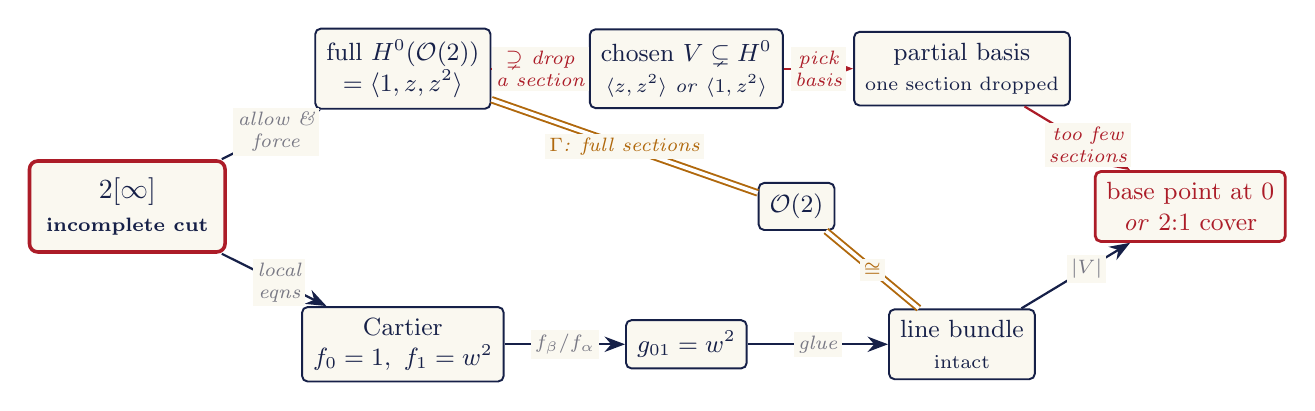
\begin{tikzpicture}
  \node[centernode] (D)   at (0,0)     {$2[\infty]$\\ \scriptsize incomplete cut};
  \node[mapnode] (LD)  at (3.5,1.75)   {full $H^0(\OO(2))$\\ $=\langle 1,z,z^2\rangle$};
  \node[mapnode] (H0)  at (7.1,1.75)   {chosen $V\subsetneq H^0$\\ \scriptsize $\langle z,z^2\rangle$ \emph{or} $\langle 1,z^2\rangle$};
  \node[mapnode] (BAS) at (10.6,1.75)  {partial basis\\ \scriptsize one section dropped};
  \node[mapnode] (CAR) at (3.5,-1.75)  {Cartier\\ $f_0=1,\ f_1=w^2$};
  \node[mapnode] (GIJ) at (7.1,-1.75)  {$g_{01}=w^2$};
  \node[mapnode] (BUN) at (10.6,-1.75) {line bundle\\ \scriptsize intact};
  \node[mapnode] (OD)  at (8.5,0)       {$\OO(2)$};
  \node[mapnode, draw=polered, line width=1pt] (PHI) at (13.5,0)
        {\textcolor{polered}{base point at $0$}\\ \textcolor{polered}{\emph{or} $2{:}1$ cover}};
  \draw[maparrow] (D)   -- node[arrlbl,pos=0.55]{allow \&\\ force} (LD);
  \draw[maparrow] (D)   -- node[arrlbl,pos=0.55]{local\\ eqns} (CAR);
  \draw[maparrow] (CAR) -- node[arrlbl]{$f_\beta/f_\alpha$} (GIJ);
  \draw[maparrow] (GIJ) -- node[arrlbl]{glue} (BUN);
  \draw[maparrow] (BUN) -- node[arrlbl,pos=0.6]{$|V|$} (PHI);
  \draw[identrung] (LD) -- node[rimlbl,pos=0.5]{$\Gamma$: full sections} (OD);
  \draw[identrung] (OD) -- node[rimlbl,pos=0.5]{$\cong$} (BUN);
  \draw[maparrow, polered] (LD)  -- node[rimlbl,text=polered]{$\supsetneq$ drop\\ a section} (H0);
  \draw[maparrow, polered] (H0)  -- node[arrlbl,text=polered]{pick\\ basis} (BAS);
  \draw[maparrow, polered] (BAS) -- node[arrlbl,text=polered,pos=0.6]{too few\\ sections} (PHI);
\end{tikzpicture}}
\end{center}
{\centering\footnotesize\itshape Map E: the bottom rail and the sheaf $\OO(2)$
stay intact (amber rungs hold). The whole failure is the single
\textcolor{polered}{red} step $H^0\supsetneq V$ --- dropping a section --- which
propagates into a base point ($V_{\mathrm{bp}}$) or a $2{:}1$ cover
($V_{\mathrm{sep}}$).\par}

\diagbox{whether base-point-freeness suffices for an embedding.}{it does not:
$\langle z,z^2\rangle$ has a base point at $0$; $\langle1,z^2\rangle$ is
base-point-free yet a branched double cover.}%
{\textcolor{accent}{Not an embedding} --- completeness was doing real work.}

%=====================================================================
\section{Comparative Table}
%=====================================================================
The five instruments side by side. Rows are the targets; columns are the probes.

\begin{center}
\renewcommand{\arraystretch}{1.35}
\resizebox{\textwidth}{!}{%
\begin{tabular}{l ccccc}
\toprule
 & \textbf{A:} $-[0]$ & \textbf{B:} $[\infty]\!-\![0]$
 & \textbf{C:} $[\infty]$ & \textbf{D:} $2[\infty]$
 & \textbf{E:} sub-$|2[\infty]|$\\
\midrule
Degree $d$         & $-1$ & $0$ & $1$ & $2$ & $2$ (bundle)\\
Allowed poles      & none & $\le1$ at $\infty$ & $\le1$ at $\infty$
                   & $\le2$ at $\infty$ & $\le2$ at $\infty$\\
Forced zeros       & $\ge1$ at $0$ & $\ge1$ at $0$ & none & none
                   & E1: $\ge1$ at $0$\\
$\dim L=\ell$      & $0$ & $1$ & $2$ & $3$ & $2$ (subspace)\\
Basis              & $\varnothing$ & $z$ & $1,\,z$ & $1,\,z,\,z^2$
                   & $z,z^2$ \,/\, $1,z^2$\\
Cartier $f_0;f_1$  & $z^{-1};\,1$ & $z^{-1};\,w$ & $1;\,w$ & $1;\,w^2$ & $1;\,w^2$\\
Transition $g_{01}$& $z$ & $1$ & $w$ & $w^2$ & $w^2$\\
$\OO(D)$           & $\OO(-1)$ & $\OO$ & $\OO(1)$ & $\OO(2)$ & $\OO(2)$\\
Base points?       & --- (empty) & none & none & none
                   & \textcolor{polered}{$\{0\}$} / none\\
Projective map     & none & to a point & $[X{:}Y]\!\mapsto\![Y{:}X]$
                   & $[Y^2{:}XY{:}X^2]$ & b.p.\ / $[Y^2{:}X^2]$ ($2{:}1$)\\
\midrule
Geometric role     & the void & collapse & iso & conic & incompleteness\\
                   & \textcolor{polered}{$H^0=0$} & \textcolor{inkblue}{trivial bundle}
                   & \textcolor{zerogreen}{$\OO(1)$ ample} & \textcolor{zerogreen}{Veronese}
                   & \textcolor{accent}{b.p.\ / cover}\\
\bottomrule
\end{tabular}}
\end{center}

%=====================================================================
\section{The Computational Pipeline}\label{sec:diagram}
%=====================================================================
Every target above is \emph{generated by the divisor} along two rails that are
welded by the invertible sheaf. \textbf{Blue single arrows are constructions}
(``build the next object from this one''); \textbf{amber double rungs are
identifications} (``the same object in another language''). The top-left arrow
``allow \& force'' is literally the valuation inequalities $\ord_p(f)+n_p\ge0$ of
Target~1.

\probemap
  {$D$}
  {$\OO(D)$}
  {line bundle $L_D$\\ \scriptsize $U_\alpha\!\times\!\CC$ glued}
  {$g_{\alpha\beta}$\\ \scriptsize cocycle}
  {Cartier\\ $(U_\alpha,f_\alpha)$}
  {$L(D)$}
  {$H^0(X,\OO(D))$}
  {basis\\ $s_0,\dots,s_r$}
  {$\Phi_D\colon X\to\PP^{r}$}

\noindent
\emph{Top rail (analytic):} $D\rightsquigarrow$ valuation inequalities
$\rightsquigarrow L(D)=H^0\to$ basis $\to\Phi_D$. \emph{Bottom rail (local):}
$D\to$ Cartier equations $f_\alpha\to g_{\alpha\beta}=f_\beta/f_\alpha\to\OO(D)\to$
line bundle. The keystone $\OO(D)$ identifies $\Gamma=H^0$ with the holomorphic
sections of the bundle, and both rails terminate in the same $\Phi_D$ --- once as
$[s_0:\cdots:s_r]$, once as the map of the complete system $|D|$.

%=====================================================================
\section{Final Synthesis}
%=====================================================================
\philobox{A divisor is a way of interrogating a geometric situation, and the
ledger is the transcript of the interrogation. Each abstract target was forced
back to arithmetic: the divisor became valuation inequalities; $L(D)$ became an
explicit space of rational functions; $\OO(D)$ became local equations
$f_\alpha=t_p^{\,n_p}$; the bundle became a single monomial transition
$g_{01}=z^{-d}$; the sections became local representatives $a_\alpha=f_\alpha s$
that are honest to the trivialization; and the map became homogeneous
polynomials whose common zeros (or absence thereof) decided base points and
embeddings. Read across the five probes, the same machinery yields nothing
($\OO(-1)$), a point ($\OO$), a line ($\OO(1)$), a conic ($\OO(2)$), and --- once
we drop a section --- a base point or a fold. To choose a divisor is to choose a
question; to run its ledger is to receive the answer in the curve's own
arithmetic.}

\end{document}
